\documentclass[landscape,9pt]{beamer}                           % COMANDI INIZIALI
\usepackage[italian]{babel}                             % sillabazione italiana
\usepackage[utf8]{inputenc}                             % Per le lettere accentate IN UNIX E IN WINDOWS
\usepackage{ragged2e}                                   % giustifica
\usepackage{amsmath}                                    % Per allineare le equazioni
\usepackage{amssymb}                                    % Per le lettere dell'indicatrice (mathbb)
\usepackage{graphicx}                                   % Per le figure
\usepackage{bm}
\usepackage{subfigure}
\usepackage{multicol}
\usepackage{animate}
\usepackage[export]{adjustbox}
\usepackage{array,multirow,graphicx}
\usepackage[misc,geometry]{ifsym}
%\usepackage{cm-super}

\renewcommand{\fontsubfuzz}{1.1pt}                          % Elimina i warning inutili

\justifying                                         % giustifica

\usetheme{CambridgeUS}
\date{29 Aprile 2015}
\author{Gabriele Mazza}
\title{Regressione con regolarizzazioni differenziali per dati spazio-temporali, con applicazione all'analisi della produzione di rifiuti urbani nella provincia di Venezia}

\makeatletter
\setbeamertemplate{footline}
{
  \leavevmode%
  \hbox{%
  \begin{beamercolorbox}[wd=.5\paperwidth,ht=2.25ex,dp=1ex,center]{author in head/foot}%
    \usebeamerfont{author in head/foot}\insertshortauthor\expandafter\beamer@ifempty\expandafter{\beamer@shortinstitute}{}{~~(\insertshortinstitute)}
  \end{beamercolorbox}%
  \begin{beamercolorbox}[wd=.5\paperwidth,ht=2.25ex,dp=1ex,right]{date in head/foot}%
    \usebeamerfont{date in head/foot}\insertshortdate{}\hspace*{2em}
    \insertframenumber{} / \inserttotalframenumber\hspace*{2ex} 
  \end{beamercolorbox}}%
  \vskip0pt%
}
\makeatother
\setbeamercolor{date in head/foot}{use=frametitle, bg=frametitle.bg}
\setbeamercolor{subsection in head/foot}{use=framtitle, bg=frametitle.bg}

\begin{document}

\begin{frame}
\maketitle
\begin{center}

\includegraphics[width=0.25\textwidth,
	height=0.28\textheight]
	{Immagini/Logo.png}
\end{center}
\end{frame}

\section{Introduzione}
\begin{frame}
\frametitle{Introduzione}
In questo lavoro di tesi è costruito e analizzato il modello di \textit{Regressione Spazio-Temporale con Penalizzazioni Differenziali} (ST-PDE) per dati distribuiti in spazio e tempo.
\par\bigskip
L'applicazione scelta riguarda l'analisi della produzione di rifiuti urbani nella provincia di Venezia tra il 1997 e il 2011
\begin{figure}[h]
	\centering
	\uncover<2->
	{
		\subfigure
   		{
		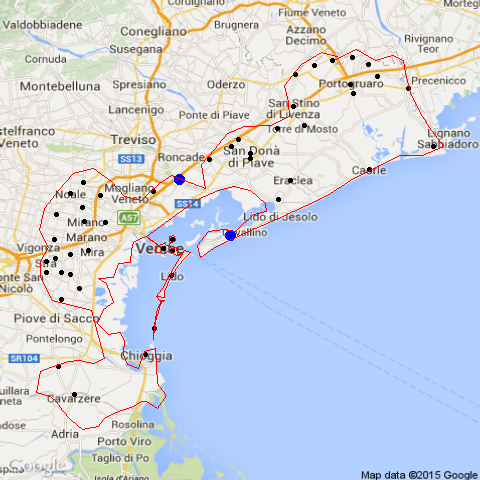
\includegraphics[width=0.40\textwidth]{Immagini/CTQDA.png}   
   		}
   	}
	\uncover<2->
	{
	\subfigure
   		{
		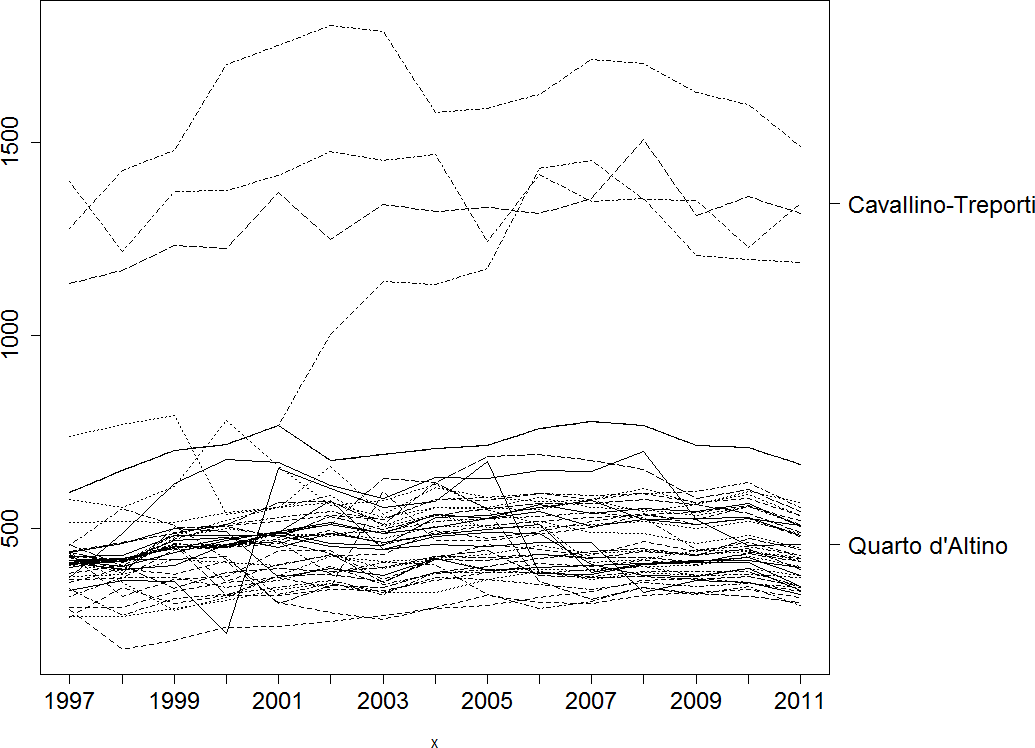
\includegraphics[width=0.43\textwidth]{Immagini/andamenti_temporali.png}
   		}
   	}
\end{figure}
\end{frame}



\section{Presentazione modello ST-PDE}
\subsection{Caso senza covariate}
\begin{frame}
\frametitle{Presentazione modello ST-PDE}
Definisco:
\begin{itemize}
\item $\{\bm{p}_i = (x_i,y_i); i=1, \ldots , n\} \subset \Omega \subset \mathbb{R}^2$
\item $\{t_j ; j=1, \ldots , m\} \subset [T_1,T_2]\subset \mathbb{R}$
\item $z_{ij}$ osservazioni in $(\bm{p}_i,t_j)$
\end{itemize}
\par\bigskip
\uncover<2->
{
	Modello:
	$$
	z_{ij}=f(\bm{p}_i,t_j)+\varepsilon_{ij}\ \ \ \ i = 1,\ldots,n\ \ j=1,\ldots,m \ \ 
	$$
	\ \ 
	\newline
	$\varepsilon_{ij}$ rumore iid di media nulla e varianza $\sigma^2$.
	
}
\uncover<3->
{
\par\bigskip
Se $\{ \psi_l(\bm{p});l = 1, \ldots , N \}$ sono basi spaziali definite in $\Omega$ e $\{ \varphi_k(t);k = 1, \ldots , M \}$ basi temporali definite in $[T_1,T_2]$, allora:
	$$
f(\bm{p}, t) = \sum_{k=1}^M a_k(\bm{p})\varphi_k(t) = \sum_{l=1}^N b_l(t)\psi_l(\bm{p}) = \sum_{l=1}^N 	\sum_{k=1}^M c_{lk}\psi_l(\bm{p})\varphi_k(t)
	$$
}
\end{frame}


\begin{frame}
Se $\{ \psi_l(\bm{p});l = 1, \ldots , N \}$ sono basi spaziali definite in $\Omega$ e $\{ \varphi_k(t);k = 1, \ldots , M \}$ basi temporali definite in $[T_1,T_2]$, allora:
	$$
f(\bm{p}, t) = \sum_{k=1}^M \textcolor<3->{red}{a_k(\bm{p})}\varphi_k(t) = \sum_{l=1}^N \textcolor<3->{red}{b_l(t)}\psi_l(\bm{p}) = \sum_{l=1}^N 	\sum_{k=1}^M c_{lk}\psi_l(\bm{p})\varphi_k(t)
	$$

La soluzione si ricaverà minimizzando il funzionale di penalizzazione:
\uncover<2->{
\begin{multline*}
J_{\bm \lambda }(f)=\sum_{i=1}^n \sum_{j=1}^m \bigl( z_{ij} - f(\bm p_i,t_j) \bigr)^2 \ + \only<2>{ \lambda_S  [\mbox{reg. spaziale}] + \lambda_T [\mbox{reg. temporale}]} \only<3->{
\lambda_S  \sum_{k=1}^M \int_{\Omega} \Bigl( \Delta(  \textcolor<3->{red}{a_k(\bm p)}  ) \Bigr)^2 d \bm p + \lambda_T \sum_{l=1}^N\int_{T_1}^{T_2} \Bigl( \frac{\partial^2  \textcolor<3->{red}{b_l(t)}   }{\partial t ^2} \Bigr)^2 dt 
}
\end{multline*}
}
\uncover<3->
{
\par\bigskip
Approccio considerato anche in Marra et al (2012).
}
\end{frame}

\begin{frame}
\only<1>
{
\begin{multline*}
J_{\bm \lambda }(f)=\sum_{i=1}^n \sum_{j=1}^m \bigl( z_{ij} - f(\bm p_i,t_j) \bigr)^2 \ +\lambda_S  \sum_{k=1}^M \int_{\Omega} \Bigl( \Delta(  \textcolor<3->{red}{a_k(\bm p)}  ) \Bigr)^2 d \bm p + \lambda_T \sum_{l=1}^N\int_{T_1}^{T_2} \Bigl( \frac{\partial^2  \textcolor<3->{red}{b_l(t)}   }{\partial t ^2} \Bigr)^2 dt 
\end{multline*}
}
\only<2->
{
$$
J_{\bm \lambda }(\bm c) = (\bm z - B \bm c)^T (\bm z - B \bm c) + \bm c^T \only<2-3>{[\lambda_S\    (P_S \otimes I_M)   \ +\  \lambda_T\   (I_N \otimes P_T)]} \only<4-5>{P}\bm c
$$
}
\uncover<3->
{
dove:
$$
\bm{c} =
\begin{bmatrix}
c_{11}  \\
\vdots\\
c_{1M}  \\
c_{21}  \\
\vdots\\
c_{NM}
\end{bmatrix}
\qquad
\bm \psi =
\begin{bmatrix}
\psi_{1}  \\
\psi_{2}  \\
\vdots\\
\psi_{N}
\end{bmatrix}
\qquad
\bm \psi_x=  \begin{bmatrix}
\partial \psi_{1}/\partial x \\
\partial \psi_{2}/\partial x  \\
\vdots\\
\partial \psi_{N}/\partial x \end{bmatrix} 
\qquad
\bm \psi_y=  \begin{bmatrix}
\partial \psi_{1}/\partial y  \\
\partial \psi_{2}/\partial y  \\
\vdots\\
\partial \psi_{N}/\partial y\end{bmatrix}
\qquad
\bm z =
\begin{bmatrix}
z_{11}  \\
\vdots\\
z_{1m}  \\
z_{21}  \\
\vdots\\
z_{nm}
\end{bmatrix}
$$
\ \ 
\newline
e le matrici: 
\begin{itemize}
\item $P_S=R_1 R_0^{-1} R_1 \qquad R_0 = \int_\Omega \bm \psi \bm \psi^T d \bm p \ , R_1 = \int_\Omega (\bm \psi_x \bm \psi_x^T + \bm \psi_y \bm \psi_y^T)d \bm p$ (Sangalli et al (2013))
\item $P_T|_{k_1,k_2} =\int_{T_1}^{T_2} \varphi_{k_1}''(t) \varphi_{k_2}''(t) dt$
\item $B = \Psi \otimes \Phi \qquad \Psi|_{i,l}=\psi_{l}(\bm p_i) \ , \Phi|_{j,k}=\varphi_{k}( t_j)$
\end{itemize}
}
\par\bigskip
\uncover<5->
{
$$
\boxed{\hat  {\bm c} = (B^T B + P)^{-1}B^T \bm z}
\qquad
\hat  {\bm z} = B(B^T B + P)^{-1}B^T \bm z = S\bm z
$$
}
\end{frame}


\subsection{Caso con covariate}
\begin{frame}
Si inseriscono nel modello $p$ possibili covariate:
$$
z_{ij}=\only<2->{\textcolor{red}{\bm w_{ij}^T \bm{\beta}} + } f(\bm{p}_i,t_j)+\varepsilon_{ij}\ \ \ \ i = 1,\ldots,n\ \ j=1,\ldots,m \ \ 
$$
$$
J_{\bm \lambda }(\bm c) = (\bm z \only<2->{\textcolor{red}{- W \bm \beta}} - B \bm c)^T (\bm z \only<2->{\textcolor{red}{- W \bm \beta}} - B \bm c) + \bm c^T S \bm c
$$
\uncover<3->
{
Derivando si trova la soluzione:
$$
\boxed{\begin{cases}
\hat{\bm \beta} = (W^TW)^{-1}W^T(\bm z - B \hat{\bm c}) \\
\hat  {\bm c} = AQ \bm z
\end{cases}}
$$
con $Q=I-W(W^TW)^{-1}W^T $ e $A=[B^TQB+P]^{-1}B^T$.
\par\bigskip
}
\uncover<4->
{
Si possono ricavare le proprietà statistiche degli stimatori:
$$
\mathbb{E}[\hat  {\bm \beta}] = \bm \beta + (W^TW)^{-1}W^T(I-B AQ)B\bm c
$$
$$
\mathrm{Var}[\hat  {\bm \beta}] = \sigma^2 (W^TW)^{-1} + \sigma^2 (W^TW)^{-1}W^T B A Q A^T B^T W(W^TW)^{-1}
$$
}
\end{frame}


\begin{frame}
Dopo aver sviluppato il modello, si scelgono le funzioni di base in spazio e tempo:
\begin{figure}[t]
	\centering
	\subfigure
	{
	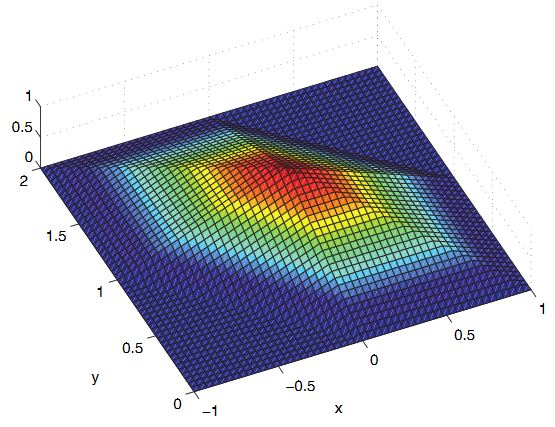
\includegraphics[width=0.46\textwidth]{Immagini/elementofinito.jpg}  
   }
	\subfigure
   {
	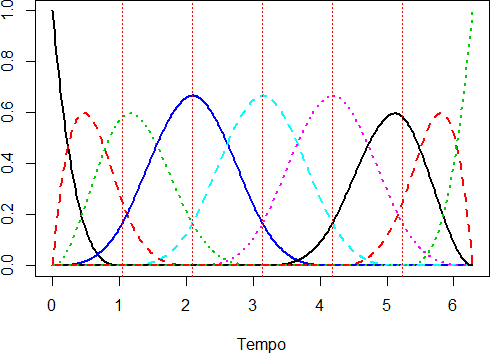
\includegraphics[width=0.46\textwidth]{Immagini/Bsplines.png}
   }
\end{figure}
\uncover<2->
{
	Per fissare i parametri di smoothing $\lambda_S$ e $\lambda_T$, si minimizza il seguente indice:
$$
\mathrm{GCV}(\bm \lambda) =\frac{nm}{nm-\text{tr}(S)}  (\bm z - \hat  {\bm z})^T(\bm z - \hat  {\bm z})
$$
}

\end{frame}

\section{Studi di simulazione}
\begin{frame}
\frametitle{Studi di simulazione}
\begin{columns}
	\begin{column}{0.6\textwidth}
	Le simulazioni sono state eseguite simulando da $f(\bm{p},t)=g(\bm{p})cos(t)$, con aggiunta del rumore:
	$$
	z_{ij}=f(\bm p_{i},t_j) + \beta w_{ij} + \varepsilon_{ij} \qquad \forall i , \forall j 
	$$
	dove:
	\begin{itemize}
	\item $\beta=1$
	\item $w_{ij}\stackrel{\mathrm{iid}}{\sim}N(0,1) \qquad \forall i, \forall j$
	\item $\varepsilon_{ij}\stackrel{\mathrm{iid}}{\sim}N(0,0.5^2) \qquad \forall i, \forall j$
	\end{itemize}
	\end{column}
	\begin{column}{0.4\textwidth}
		\begin{center}
		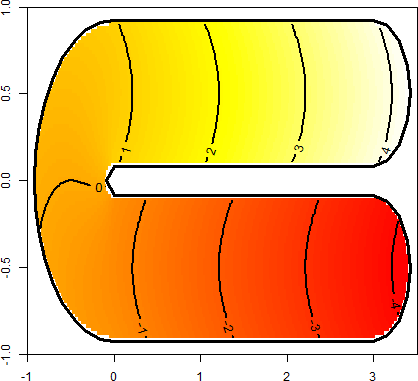
\includegraphics[width=0.8\textwidth]{Immagini/DomC_fstest.png}
		\end{center}
		\begin{center}
		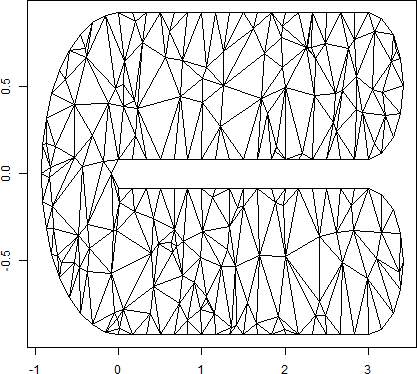
\includegraphics[width=0.8\textwidth]{Immagini/DomC_Triangolazione.png}
		\end{center}
	\end{column}
\end{columns}
\end{frame}

\subsection{Caso con covariata}
\begin{frame}
\begin{columns}
	\begin{column}{0.25\textwidth}
	Il modello stima:
	$$
	\hat{\beta} \approx 1.001 
	$$
	IC approssimato:
	$$
	\beta \in [0.9809;1.0225]
	$$
	\end{column}
	\begin{column}{0.65\textwidth}	
		\begin{flushright}		
		\animategraphics[autoplay,loop,height=5cm]{5}{Immagini/AnimazioneCovar/image}{1}{100}
		\end{flushright}
	\end{column}
\end{columns}
\end{frame}


\section{Confronto con altri metodi}
\subsection{Caso senza covariata}
\begin{frame}
\frametitle{Confronto con altri metodi}
\begin{columns}
	\begin{column}{0.6\textwidth}
	L'algoritmo è stato confrontato con altre tecniche già esistenti:
	\begin{itemize}
	\item<2-> KRIG: modello basato su kriging spazio-temporale (Caballero et al (2013),
Menafoglio et al (2013) and Menafoglio et al (2014))
	\item<3-> TPS: basi in spazio \textit{Thin Plate Splines} (Wood (2003)), in tempo \textit{Smoothing Splines}
	\item<4-> SOAP: basi in spazio \textit{Soap Film Smoothing} (Wood et al (2008)), in tempo \textit{Smoothing Splines} 
	\end{itemize}
	\uncover<5->
	{Solo SOAP e ST-PDE possono tener conto del dominio spaziale.}
	\end{column}
	\begin{column}{0.4\textwidth}
	\uncover<6->
	{\begin{flushright}
		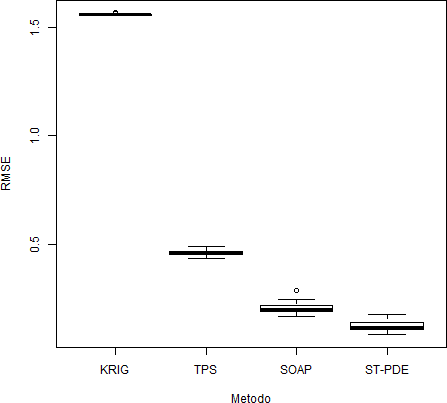
\includegraphics[width=1\textwidth]{Immagini/Confronto_metodi.png}
	\end{flushright}}		
	\end{column}
\end{columns}
\end{frame}

\begin{frame}
\begin{figure}
\centering
\begin{tabular}{lccccc}
& Reale & KRIG & TPS & SOAP & ST-PDE \\
\parbox[t]{2mm}{\multirow{3}{*}{\rotatebox[origin=r]{90}{$t=0$}}}&
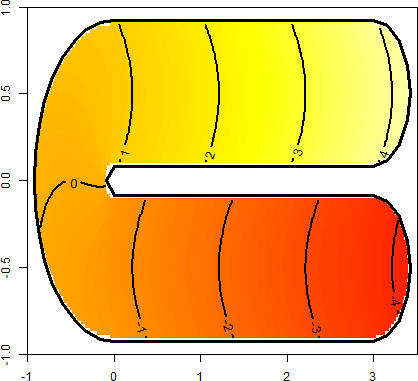
\includegraphics[width=0.16\textwidth,valign=t]{Immagini/simulazioni/REALEtempo1.png} &
\uncover<2->{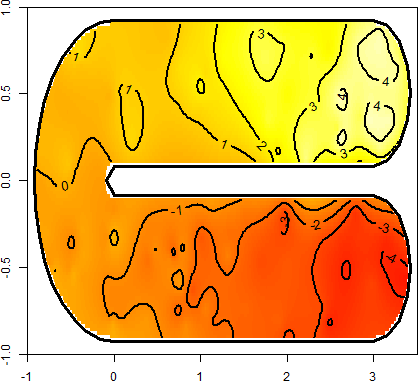
\includegraphics[width=0.16\textwidth,valign=t]{Immagini/simulazioni/KRIGtempo1.png}}&
\uncover<3->{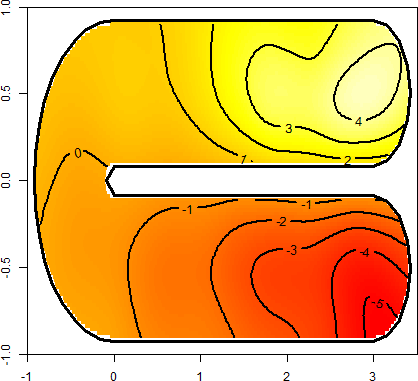
\includegraphics[width=0.16\textwidth,valign=t]{Immagini/simulazioni/TPStempo1.png}}&
\uncover<4->{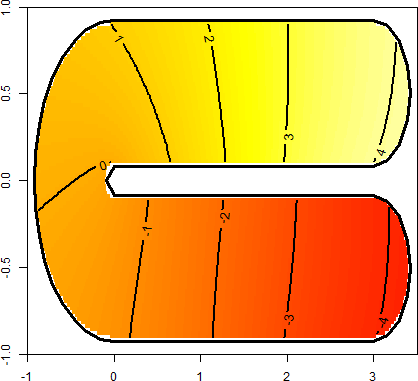
\includegraphics[width=0.16\textwidth,valign=t]{Immagini/simulazioni/SOAPtempo1.png}}&
\uncover<5->{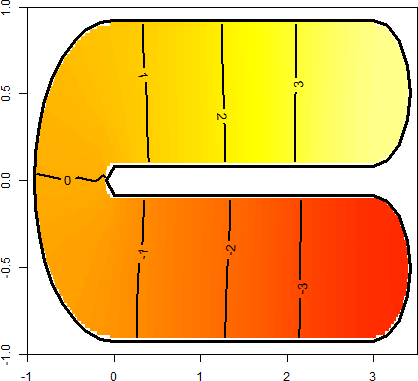
\includegraphics[width=0.16\textwidth,valign=t]{Immagini/simulazioni/STSRtempo1.png}}\\
\parbox[t]{2mm}{\multirow{3}{*}{\rotatebox[origin=c]{90}{$t=\frac{\pi}{4}$}}}&
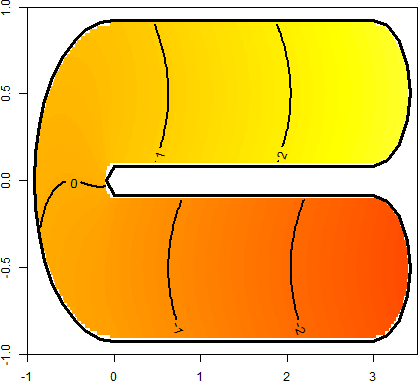
\includegraphics[width=0.16\textwidth,valign=t]{Immagini/simulazioni/REALEtempo2.png}&
\uncover<2->{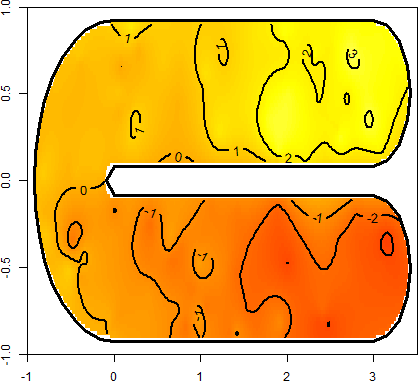
\includegraphics[width=0.16\textwidth,valign=t]{Immagini/simulazioni/KRIGtempo2.png}}&
\uncover<3->{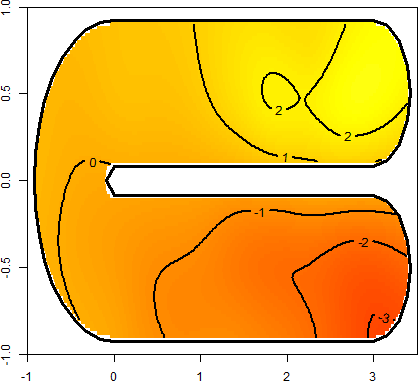
\includegraphics[width=0.16\textwidth,valign=t]{Immagini/simulazioni/TPStempo2.png}}&
\uncover<4->{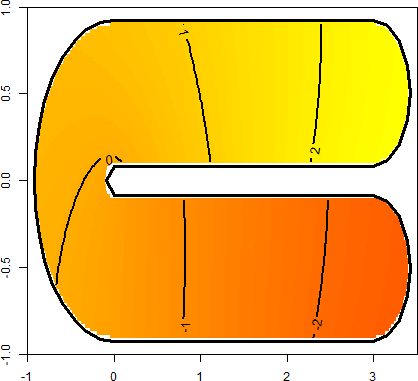
\includegraphics[width=0.16\textwidth,valign=t]{Immagini/simulazioni/SOAPtempo2.png}}&
\uncover<5->{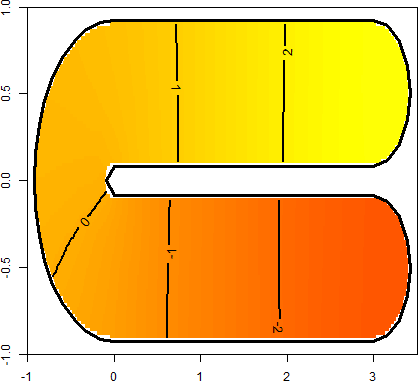
\includegraphics[width=0.16\textwidth,valign=t]{Immagini/simulazioni/STSRtempo2.png}}\\
\parbox[t]{2mm}{\multirow{3}{*}{\rotatebox[origin=c]{90}{$t=\frac{\pi}{2}$}}}&
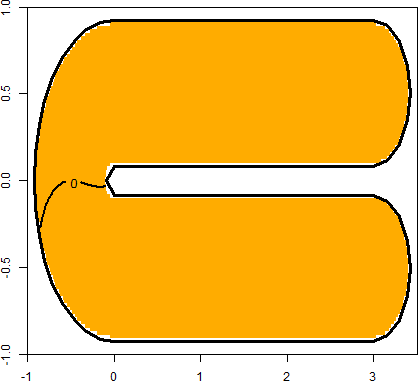
\includegraphics[width=0.16\textwidth,valign=t]{Immagini/simulazioni/REALEtempo3.png}&
\uncover<2->{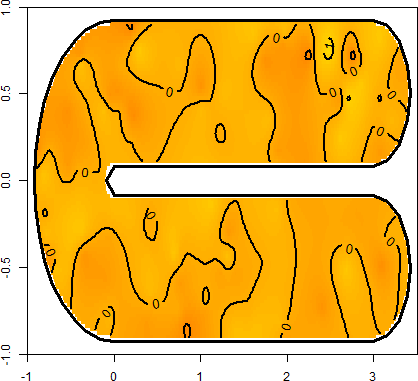
\includegraphics[width=0.16\textwidth,valign=t]{Immagini/simulazioni/KRIGtempo3.png}}&
\uncover<3->{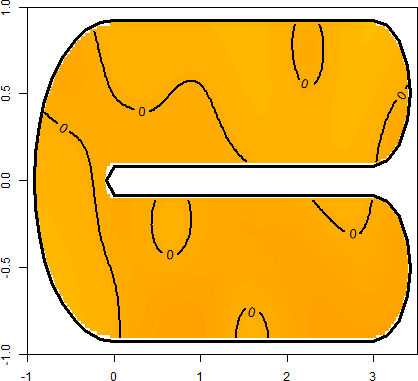
\includegraphics[width=0.16\textwidth,valign=t]{Immagini/simulazioni/TPStempo3.png}}&
\uncover<4->{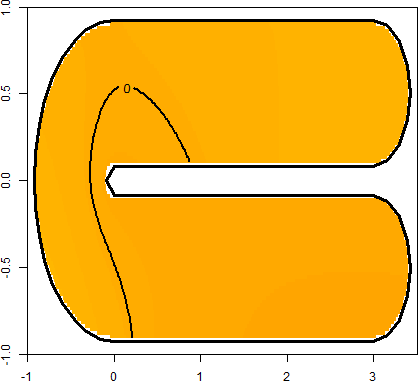
\includegraphics[width=0.16\textwidth,valign=t]{Immagini/simulazioni/SOAPtempo3.png}}&
\uncover<5->{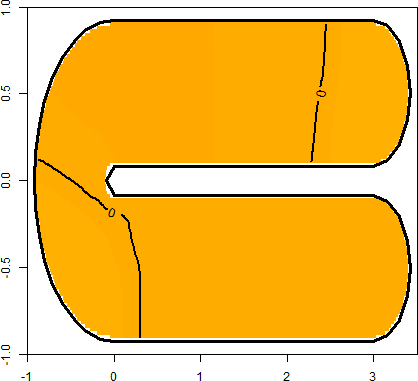
\includegraphics[width=0.16\textwidth,valign=t]{Immagini/simulazioni/STSRtempo3.png}}\\
\parbox[t]{2mm}{\multirow{3}{*}{\rotatebox[origin=c]{90}{$t=\frac{3}{4}\pi$}}}&
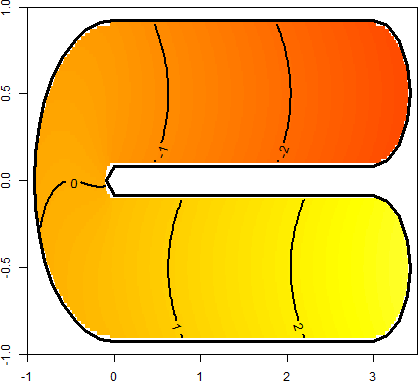
\includegraphics[width=0.16\textwidth,valign=t]{Immagini/simulazioni/REALEtempo4.png}&
\uncover<2->{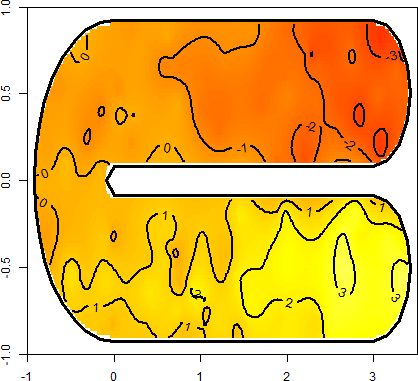
\includegraphics[width=0.16\textwidth,valign=t]{Immagini/simulazioni/KRIGtempo4.png}}&
\uncover<3->{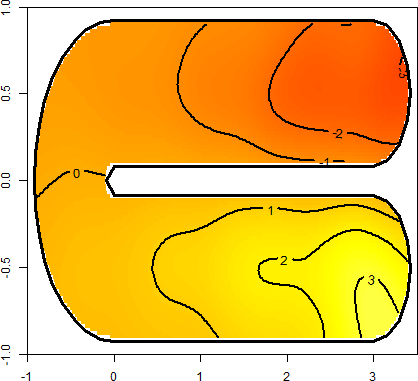
\includegraphics[width=0.16\textwidth,valign=t]{Immagini/simulazioni/TPStempo4.png}}&
\uncover<4->{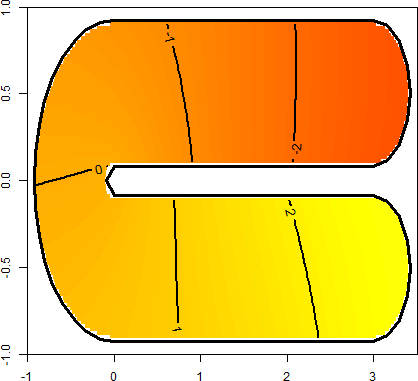
\includegraphics[width=0.16\textwidth,valign=t]{Immagini/simulazioni/SOAPtempo4.png}}&
\uncover<5->{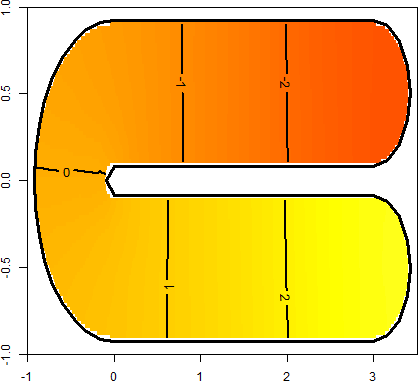
\includegraphics[width=0.16\textwidth,valign=t]{Immagini/simulazioni/STSRtempo4.png}}
\end{tabular}
\end{figure}
\end{frame}

\subsection{Caso con covariata}
\begin{frame}
I confronti dei metodi sono stati eseguiti anche nel caso con covariata (senza il kriging):
\par\bigskip
\begin{figure}[h]
	\centering
		\subfigure
   		{
		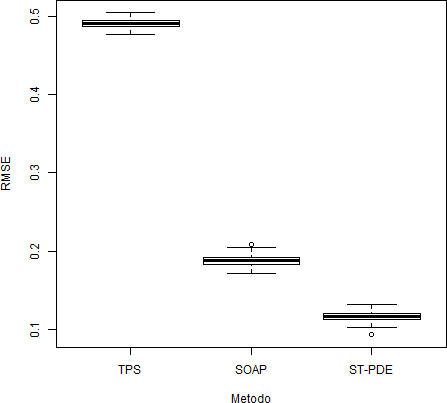
\includegraphics[width=0.40\textwidth]{Immagini/Confronto_metodi_covar.png}   
   		}
	\subfigure
   		{
		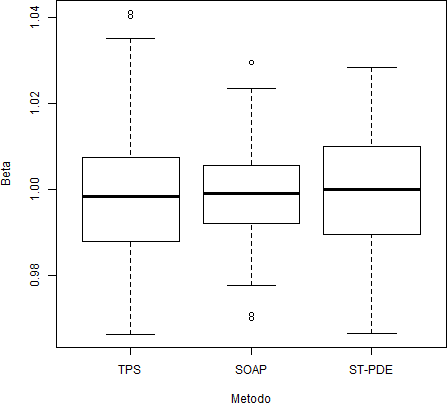
\includegraphics[width=0.43\textwidth]{Immagini/Confronto_metodi_beta.png}
   		}
\end{figure}
\end{frame}

\section{Applicazione allo studio dei rifiuti nella provincia di Venezia}

\begin{frame}
\frametitle{Applicazione allo studio dei rifiuti nella provincia di Venezia}
\begin{columns}
	\begin{column}{0.6\textwidth}
	I dati sono stati localizzati in un unico punto, nel paese di riferimento del comune.
	\newline\newline
	Come covariata, per tener conto dell'effetto del turismo, si usa il numero di posti letto pro capite in strutture ricettive.
	\newline\newline
	Sono stati usati i valori pro capite, sia per il dato che per la covariata (possibilità di replicare i dati poichè densità).
		I parametri di smoothing sono calcolati tramite GCV.

	\end{column}
	\begin{column}{0.4\textwidth}
	\begin{center}
		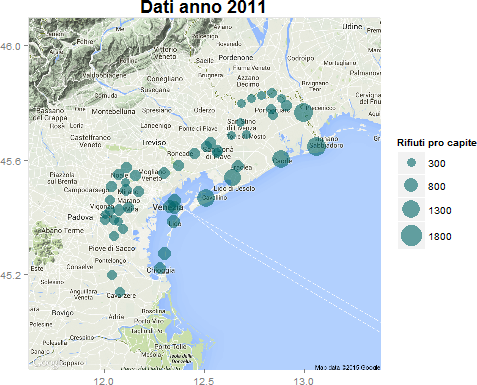
\includegraphics[width=0.8\textwidth]{Immagini/Dati.png}
	\end{center}
	\begin{center}
		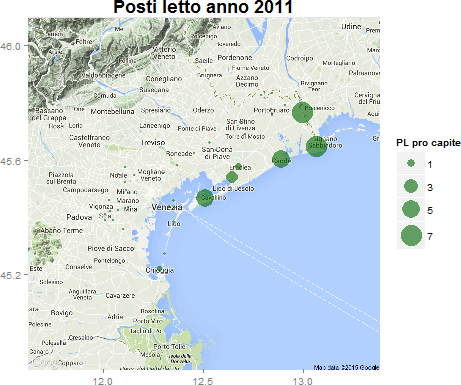
\includegraphics[width=0.8\textwidth]{Immagini/PL.png}
	\end{center}		
	\end{column}
\end{columns}
\end{frame}

\subsection{Caso con covariata}
\begin{frame}
Risultati dell'applicazione del modello con la covariata:
$$
\hat{\beta}\approx 30.5563 \qquad \beta \in [14.3158;46.7767]
$$
\begin{columns}
	\begin{column}{0.45\textwidth}
	\begin{figure}
	\begin{multicols}{2}
	\centering
	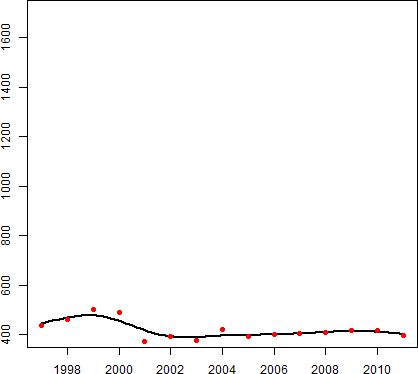
\includegraphics[width=0.45\textwidth]{Immagini/VeneziaCovar/Cavarzere.png}\\
	Cavarzere 
	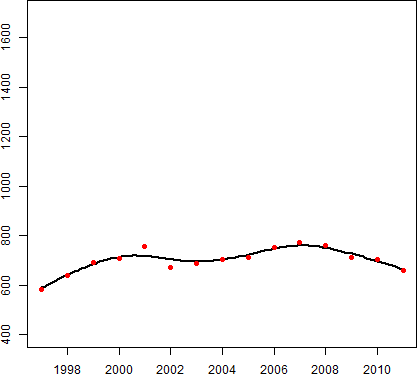
\includegraphics[width=0.45\textwidth]{Immagini/VeneziaCovar/Venezia.png}\\
	Venezia 
	\end{multicols}
	\begin{multicols}{2}
	\centering
	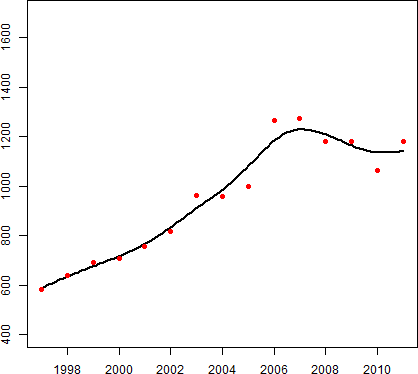
\includegraphics[width=0.45\textwidth]{Immagini/VeneziaCovar/Cavallino-Treporti.png}\\
	Cavallino-Treporti
	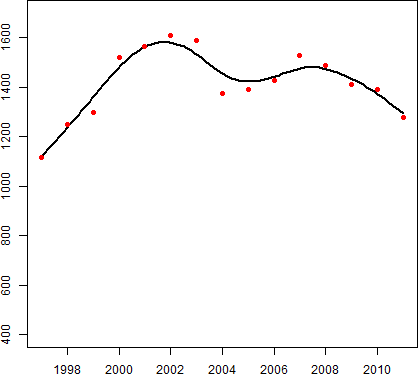
\includegraphics[width=0.45\textwidth]{Immagini/VeneziaCovar/Bibione.png}\\
	Bibione
	\end{multicols}
	\end{figure}
	\end{column}
	
	\begin{column}{0.35\textwidth}	
		\begin{center}		
		\animategraphics[autoplay,loop,height=4.5cm,width=4cm]{10}{Immagini/VeneziaCovar/image}{1}{100}
		\end{center}
	\end{column}
\end{columns}
\end{frame}

\section{Sviluppi futuri}
\begin{frame}
\frametitle{Sviluppi futuri}
Il modello ST-PDE può essere ulteriormente sviluppato, per poter essere applicato ad ulteriori casi:
\begin{itemize}
\item<2-> è possibile riferire i dati ad un'area, e non ad un punto? Modello per il caso areale (in corso)
\item<3-> miglioramenti computazionali, per avere un codice più efficiente ed applicabile a dataset più grandi
\end{itemize}

\end{frame}

\section{Bibliografia}
\begin{frame}
\frametitle{Bibliografia}

N.H. Augustin, V.M. Trenkel, S.N. Wood, P. Lorance, \emph{Space-time modelling of blue ling for fisheries stock management}, Environmetrics, 24, pp. 109–119, 2013.
\par\bigskip
W. Caballero, R. Giraldo, J. Mateu, \emph{A universal kriging approach for spatial functional data}, Stochastic Environmental Research and Risk Assessment 27(7), pp. 1553-1563, Springer, 2013.
\par\bigskip
G. Marra, D.L. Miller, Luca Zanin, \emph{Modelling the spatiotemporal distribution of the incidence of resident foreign population}, Statistica Neerlandica, 66, pp. 133–160, 2012.
\par\bigskip
A. Menafoglio, A. Guadagnini, P. Secchi, \emph{A kriging approach based on Aitchison geometry for the characterization of particle-size curves in heterogeneous aquifers}, Stochastic Environmental Research and Risk Assessment, 28(7), pp. 1835-1851, 2014.
\par\bigskip
\begin{flushright}
[segue]
\end{flushright}
\end{frame}

\begin{frame}
\frametitle{Bibliografia}

A. Menafoglio, P. Secchi, M. Dalla Rosa et al., \emph{A Universal Kriging predictor for spatially dependent functional data of a Hilbert Space}, Electronic Journal of Statistics, 7, pp. 2209-2240, 2013.
\par\bigskip
L.M. Sangalli, J.O. Ramsay, T.O. Ramsay, \emph{Spatial spline regression models}, Journal of the Royal Statistical Society, Series B, 75, pp. 681–703, 2013.
\par\bigskip
S.N. Wood, \emph{Thin-plate regression splines}, Journal of the Royal Statistical Society (B), 65(1), pp. 95-114, 2003.
\par\bigskip
S.N. Wood, M.W. Bravington, S.L. Hedley, \emph{Soap film smoothing}, Journal of the Royal Statistical Society, Series B, 70, pp. 931–955, 2008.

\end{frame}

\end{document}